\documentclass[border=6pt]{standalone}
\usepackage{tikz}
\usetikzlibrary{arrows.meta,calc,positioning}
\begin{document}
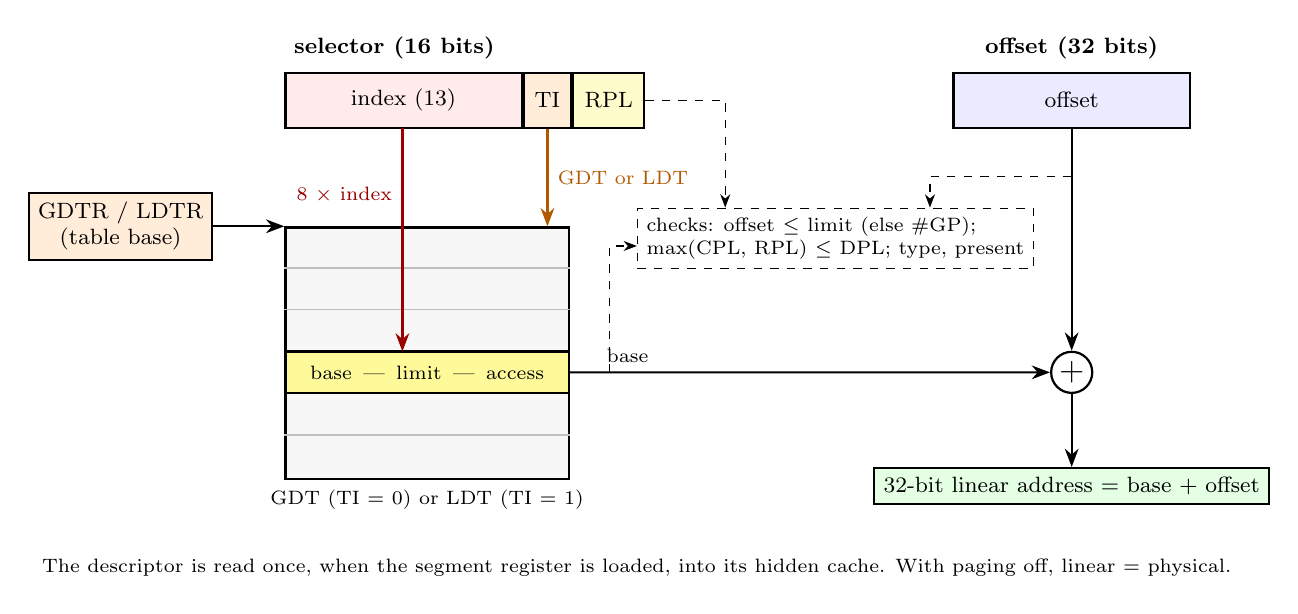
\begin{tikzpicture}[>=Stealth,font=\small,
 fld/.style={draw,thick,minimum height=0.7cm,align=center,font=\footnotesize}]
% selector and offset
\node[font=\footnotesize\bfseries,anchor=south west] at (0,0.4) {selector (16 bits)};
\node[fld,minimum width=3.0cm,fill=red!8,anchor=west] (idx) at (0,0) {index (13)};
\node[fld,minimum width=0.6cm,fill=orange!15,right=0pt of idx] (ti) {TI};
\node[fld,minimum width=0.9cm,fill=yellow!20,right=0pt of ti] (rpl) {RPL};
\node[font=\footnotesize\bfseries,anchor=south] at (10.0,0.4) {offset (32 bits)};
\node[fld,minimum width=3.0cm,fill=blue!8] (off) at (10.0,0) {offset};
% descriptor table under the selector
\node[draw,thick,fill=gray!6,minimum width=3.6cm,minimum height=3.2cm,anchor=north west] (tab) at (0,-1.6) {};
\node[font=\scriptsize,anchor=north] at (tab.south) {GDT (TI = 0) or LDT (TI = 1)};
\foreach \k in {1,...,5} \draw[gray!50] ($(tab.north west)+(0,-\k*0.53)$) -- ($(tab.north east)+(0,-\k*0.53)$);
\node[draw,thick,fill=yellow!40,minimum width=3.6cm,minimum height=0.53cm,font=\scriptsize] (desc) at ($(tab.north)+(0,-1.855)$) {base\enspace|\enspace limit\enspace|\enspace access};
\node[draw,thick,fill=orange!15,font=\footnotesize,align=center,anchor=east] (gdtr) at (-0.9,-1.6) {GDTR / LDTR\\(table base)};
\draw[->,thick] (gdtr.east) -- (tab.north west);
\draw[->,thick,red!60!black] (1.5,-0.35) -- (1.5,-3.19) node[pos=0.3,left,font=\scriptsize]{8 $\times$ index};
\draw[->,thick,orange!70!black] (ti.south) -- (ti.south |- tab.north) node[pos=0.5,right,font=\scriptsize]{GDT or LDT};
% adder and linear address
\node[draw,thick,circle,inner sep=1pt,font=\large] (add) at (10.0,-3.455) {$+$};
\draw[->,thick] (desc.east) -- (add.west) node[pos=0.12,above,font=\scriptsize]{base};
\draw[->,thick] (off.south) -- (add.north);
\node[draw,thick,fill=green!10,font=\footnotesize] (lin) at (10.0,-4.9) {32-bit linear address = base + offset};
\draw[->,thick] (add.south) -- (lin.north);
% checks
\node[draw,dashed,font=\scriptsize,align=left] (chk) at (7.0,-1.75) {checks: offset $\le$ limit (else \#GP);\\max(CPL, RPL) $\le$ DPL; type, present};
\draw[->,dashed] ($(desc.east)+(0.5,0)$) |- ($(chk.west)+(0,-0.1)$);
\draw[->,dashed] (rpl.east) -| ($(chk.north)+(-1.4,0)$);
\draw[->,dashed] ($(off.south)+(0,-0.6)$) -| ($(chk.north)+(1.2,0)$);
\node[font=\scriptsize,align=left,anchor=north west] at (-3.2,-5.7) {The descriptor is read once, when the segment register is loaded, into its hidden cache. With paging off, linear = physical.};
\end{tikzpicture}
\end{document}
